\input{content/theme.tex}
\bibliography{content/bibliography}


\begin{document}


%\includepdf[pages=-]{content/titlepage.pdf}

\title{Introduction to Decision Trees}



\begin{titlepage} 
\thispagestyle{empty}


%Sustainable Energy by Benni from The Noun Project

\begin{center}
    {\fontsize{60}{60} \bfseries \textsf{Decision Trees}}\\[1em]
        
    \noindent\rule{\textwidth}{0.5pt} \\[1em]
    {\Large \textsf{An Introduction} } \\[4em]
    %\noindent\rule{\textwidth}{0.5pt} \\[3em]
    
    \includegraphics[width=0.35\textwidth]{content/decisiontree}
    
    \vspace{5em}

    {\sffamily \large \bfseries  Seminar paper for the course \textit{Artificial Intelligence} (KISEM)}\\[3em]


    {  \normalsize 
        Michael Dorner \\[2em]
        
        \today

    } 
\end{center}

\end{titlepage}


\newpage

\renewcommand{\contentsname}{Table of Content}
\tableofcontents
\vfill


\newpage


% Content

\section{Introduction}


\subsection{What is a decision tree?} \label{whatisadecisiontree}
A business student with only a very few programming skills shall develop a simple algorithm for sorting three elements $A, B, C$. He decides to divide this problem in smaller subproblems. First he wonders if $A$ is smaller then $B$. In the second step it is interesting if $B$ is smaller then $C$. If $A<B$ and $B<C$ then $A<B<C$. But if $B$ is not greater then $C$, then a third question is relevant: Is $A<C$? 

His head is spinning. Maybe solving this problem graphically is a better idea. He draws a node for each question and an edge for each answer. All leafs represent the correct order. Figure \ref{fig:sortingtree} shows the resulting graph:

\begin{figure}[!h]
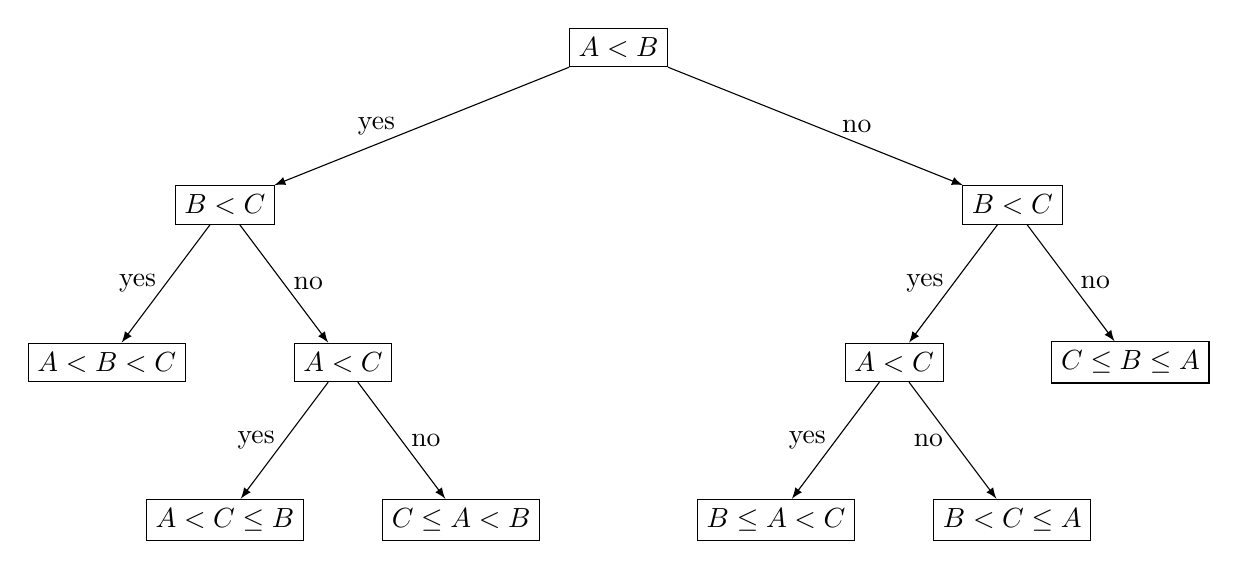
\begin{tikzpicture}[edge from parent/.style={draw,-latex},
level distance=2cm,
level 1/.style={sibling distance=10cm},
level 2/.style={sibling distance=3cm}]
\tikzstyle{every node}=[rectangle,draw]    
\node (Root) {$A < B$}
child {
    node {$B < C$}    
    child { 
        node {$A < B < C$} 
        edge from parent node[left,draw=none] {yes}
    }
    child { 
        node {$A < C$} 
        child {
            node {$A < C \leq B$}
            edge from parent node[left,draw=none] {yes}
        }
        child {
            node {$C \leq A < B$}
            edge from parent node[right,draw=none] {no}
        }
        edge from parent node[right,draw=none] {no}
    }
    edge from parent node[left,draw=none] {yes $\;$}
}
child {
    node {$B < C$}
    child { 
        node {$A < C$}     
        child {
            node {$B \leq A < C$}
            edge from parent node[left,draw=none] {yes}
        }   
        child {
            node {$B < C \leq A$}
            edge from parent node[left,draw=none] {no}
        }     
        edge from parent node[left,draw=none] {yes}
    }
    child { 
        node {$C \leq B \leq A$} 
        edge from parent node[right,draw=none] {no}
    }
    edge from parent node[right,draw=none] { $\;$ no}
};
\end{tikzpicture}
\caption{A decision tree for sorting three values.}
\label{fig:sortingtree}
\end{figure}

Without further knowledge the student created his first decision tree.

For a right decision two or three if-statements are necessary. So a Python program could look like listing \ref{lst:sort1}.

\newpage

\begin{lstlisting}[style = fau, language = Python, caption={[A Python implementation of a decision tree for sorting three elements]A Python implementation of a decision tree for sorting three elements $A, B, C$},label=lst:sort1]
def sort1(A, B, C):
	if (A < B):
		if (B < C):
			return [A, B, C]
		else:
			if (A < C):
				return [A, C, B]
			else:
				return [C, A, B]
	else:
		if (B < C):
			if (A < C):
				return [B, A, C]
			else:
				return [B, C, A]
		else:
			return [C, B, A]

print( sort1(9,-2,0) ) # >> [-2, 0, 9]
print( sort1(2,0,0) )  # >> [0, 0, 2]
\end{lstlisting}

\begin{remark}
    The Python if-statement syntax implies the tree structure in a vertical form, too.      
\end{remark}

Another way of formatting if-clauses represents a rule set which are first order logical expressions:  
    \begin{lstlisting}[style = fau, language = Python, caption={A Python reimplementation of the decision tree given in listing \ref{lst:sort1} as a set of first order logical rules},label=lst:sort2]
def sort2(A, B, C):
	if (A < B) and (B < C) : return [A, B, C]
	if (A < B) and not (B < C) and (A < C): return [A, C, B]
	if (A < B) and not (B < C) and not (A < C): return [C, A, B]
	if not (A < B) and (B < C) and (A < C): return [B, A, C]
	if not (A < B) and (B < C) and not (A < C): return [B, C, A]
	if not (A < B) and not (B < C) : return [C, B, A]
\end{lstlisting}

Unsurprisingly, we get six rules for $3! = 6$ different combinations and the same results as in the algorithm \texttt{sort1}. 


This introductory example shows four important properties: Decision trees
\begin{enumerate}
    \item work very well for classification and data mining.
    \item are intuitive and self-explanatory.
    \item are easy to implement.
    \item can be even used by business students.
\end{enumerate}

\begin{remark}
    Decision trees are used to model all comparison sorts like mergesort or quicksort. The reader may notice that the decision tree in figure \ref{fig:sortingtree} represents the insertion sort algorithm \cite[p. 208]{cormen2001introduction}. 
\end{remark}





\section{Theory of Decision Trees}

In this section a (computer) scientific base for the informal introduction of decision trees shall be given. As mentioned in the introduction a basic knowledge in graph theory, machine learning and computer science in general is assumed.


\subsection{Definitions}

\begin{definition}
A \textbf{tree} is a directed, connected graph with one root node. Every other node has a single predecessor (\textbf{parent}) and no or more successors (\textbf{children}). Nodes without successors are called \textbf{leaves}. All nodes are connected by \textbf{edges}. The \textbf{depth} of a node is the number of edges on the path to the root. The \textbf{height} of the whole tree is the number of edges on the longest path from the root to any leaf. 
\end{definition}

\begin{remark}
This very rough definition focussed on trees shall not hide the fact that graph theory is complex and enormous mathematical field. For a deeper look e.g. \cite{cormen2001introduction} is recommended.
\end{remark}

\begin{definition}
A \textbf{decision tree} is a tree with following equivalents:
\begin{center}
\begin{tabular}{l|l} 
    \textbf{Tree} &  \textbf{Decision tree equivalent} \\ \hline
    Root & Initial decision node  \\ 
    Node & Internal decision node for testing on an attribute  \\ 
    Edge & Rule to follow \\ 
    Leaf & Terminal node represents the resulting classification 
\end{tabular}
\end{center}
\end{definition}

As mentioned in subsection \ref{taxonomy}, machine learning is a set of algorithms that extract models representing patterns from data and then evaluate those models. Let us define four relevant terms, which are important for understanding the following algorithms descriptions: instance, attribute, class, and dataset:

\begin{definition}
    The input of a machine learning algorithm consists of a set of \textbf{instances} (e.g. rows, examples or observations). Each instance is described by a fixed number of \textbf{attributes} (i.e. columns), which are assumed to be either nominal or numeric, and a label which is called \textbf{class} (in case of a classification task). The set of all instances is called \textbf{dataset}.
\end{definition}

Following this definition we get a table containing the dataset: Each decision becomes an attribute (all binary relations), all leaves are classes, while each row represents an instance of the dataset (see table \ref{tab:decisiontable}).

\begin{table}[!h] \centering
\begin{tabular}{|l| l l l |l|} \hline
    \textbf{Instance} & \multicolumn{3}{c|}{\textbf{Attribute}} & \multicolumn{1}{c|}{\textbf{Class}}\\ 
    & $A<B$ & $B<C$ & $A<C$ &  \\ \hline
    1 & yes & yes & yes & $A < B < C$ \\ 
    2 & yes & yes & no & $A < B < C$ \\
    3 & yes & no & yes & $A < C \leq B$ \\
    4 & yes & no & no & $C \leq A < B$ \\
    5 & no & yes & yes & $B \leq A < C$ \\ 
    6 & no & yes & no & $B < C \leq A$ \\
    7 & no & no & yes & $C \leq B \leq A$ \\
    8 & no & no & no & $C \leq B \leq A$ \\ \hline
\end{tabular}
\caption{Dataset table for the sorting example from subsection \ref{whatisadecisiontree}}
\label{tab:decisiontable}
\end{table}

Normally, the transformation is vice versa: the data is collected in table form (e.g. databases) and a decision tree has to be generated. 

The reason why there are now eight instead of six classes is simple: it does not matter for instances 1, 2 and 7, 8, if $A<B$ or not; the result is the same class. This effect of removing irrelevant branches of a tree is called pruning and is also part of this paper (see \ref{treepruning}). 


\newpage

\subsection{Decision Tree Learning}

In this subsection the question how to generate a decision tree from a given dataset in general shall be answered.

A founding idea of tree-based classification is based in the Concept Learning System \cite{quinlan1986induction}.
All algorithms introduced in the next section are based on a simple but very powerful algorithm called TDIDT which stands for \textit{Top-Down Induction of Decision Trees} \cite{quinlan1986induction}. This algorithm framework consists of two methods, growing and pruning a decision tree, which are introduced in the next two pseudocode listings and follows the idea of divide and conquer \cite[p. 33]{cormen2001introduction}. 

\begin{remark}
    $\sigma$ is the relational operator for selection. See e.g. \cite[p. 145]{rob2008database} for further operators and more detailed information. 
\end{remark}

 
\begin{algorithm}
\SetKwInOut{Input}{Input}
\SetKwInOut{Output}{Output}
\SetKwFunction{treePruning}{treePruning}
\SetKwFunction{treeGrowing}{treeGrowing}
\SetKwFunction{stoppingCriterion}{stoppingCriterion}
\SetKwFunction{splittingCriterion}{splittingCriterion}
\Input{Training set $X$, attribute set $A$, target feature $y$}
\Output{Decision tree}
\BlankLine
Create a new tree $T$ with a single root node.\\
\eIf{\stoppingCriterion{$X$}}{
    Mark $T$ as a leaf with the most common value in $X$ as a label.
}{
    $\forall a_i \in A$ find \textcolor{faured}{$a$} that obtain the best \splittingCriterion{$a_i, X, y$}.\\
    Label $n$ with $a$.\\
    \For{each outcome \textcolor{faublue}{$v_i$} of \textcolor{faured}{$a$}}{
        Set subtree \textcolor{faugreen}{$t_i$} = \treeGrowing{$\sigma_{a=v_i}X, A, y$}. \\
        Connect the root node of $n_t$ to the subtree \textcolor{faugreen}{$t_i$} with an edge that is labelled as \textcolor{faublue}{$v_i$}.
    }
}
\Return{\treePruning{$S, T, y$}}
\caption{Tree Growing \texttt{treeGrowing}}
\end{algorithm}

\begin{algorithm}
\SetKwInOut{Input}{Input}
\SetKwInOut{Output}{Output}
\SetKwFunction{pruned}{pruned}
\Input{Training set $X$, tree to be pruned $T$, target feature $y$}
\Output{Decision tree}
\BlankLine
\Repeat{$t = \emptyset$}{
      Select a node $n$ in $T$ such that pruning this node $n$ maximally improves some evaluation criterions. \\
    \If{$n \neq \emptyset$}{
        $T = $ \pruned{$T, n$}
    }
}
\Return{$T$}
\caption{Tree Pruning \texttt{treePruning}}
\end{algorithm}


A simplified decision tree \ref{fig:frameworktree} created by this algorithmic framework shall clarify how it works. The colors correspond to the variables in the pseudocode.

\begin{figure}[!h] \centering
\begin{tikzpicture}[
    level distance=2cm,
    level 1/.style={sibling distance=2.5cm},
    level 2/.style={sibling distance=4cm},
    leaf/.style={isosceles triangle,dashed,shape border rotate=90,isosceles triangle stretches=true, minimum height=20mm,minimum width=20mm,inner sep=0,yshift={-20mm}}]
\tikzstyle{every node}=[rectangle,draw]    
\node (Root) {\textcolor{faured}{$a$}}
child[child anchor=north] { 
    node[leaf] {\textcolor{faugreen}{$t_1$}}
    edge from parent node[left,draw=none] {\textcolor{faublue}{$v_1\;$}}
}
child[child anchor=north] { 
    node[leaf] {\textcolor{faugreen}{$t_2$}}
    edge from parent node[right,draw=none] {\textcolor{faublue}{$v_2$}}
}
child[child anchor=north] { 
    node[leaf, text height=1.5em] {$\dots $}
    edge from parent node[right,draw=none] {$\dots$}
}
child[child anchor=north] { 
    node[leaf] {\textcolor{faugreen}{$t_n$}}
    child[grow=right, xshift={10mm}] {
        node[draw=none]{Subtrees}
        edge from parent[draw=none]
        child[grow=up, yshift={7.5mm}] {
            node[draw=none]{Values of \textcolor{faured}{$a$}}  
            edge from parent[draw=none]
            child[grow=up, yshift={-7.5mm}] {
                node[draw=none]{Best attribute in $A$}  
                edge from parent[draw=none]
            } 
        }    
    }
    edge from parent node[right,draw=none] {\textcolor{faublue}{$v_n$}}
}
;
\end{tikzpicture}
\caption{The basic structure of a decision tree created by the algorithmic framework.}
\label{fig:frameworktree}
\end{figure}
\input{content/conclusion.tex}


\setcounter{section}{0}
\renewcommand{\thesection}{\Alph{section}}



\newpage

\section{Bibliography}
%\addcontentsline{toc}{section}{Bibliography}
\printbibliography[heading=none]


\end{document}



